\chapter{Скачаща дъга}

Целта на играта е да се вкара топчето в купата. Играчът управлява топчето с помощта на мишката. Когато се стартира играта купата подскача от лявата част на екрана до дясната, като оставя след себе си следа, която представлява дъга. Играчът трябва да управлява топчето така че до да преминава само по дъгата. Ако не докосва дъгата - играта започва отначало.

\begin{figure}[H]
  \centering
  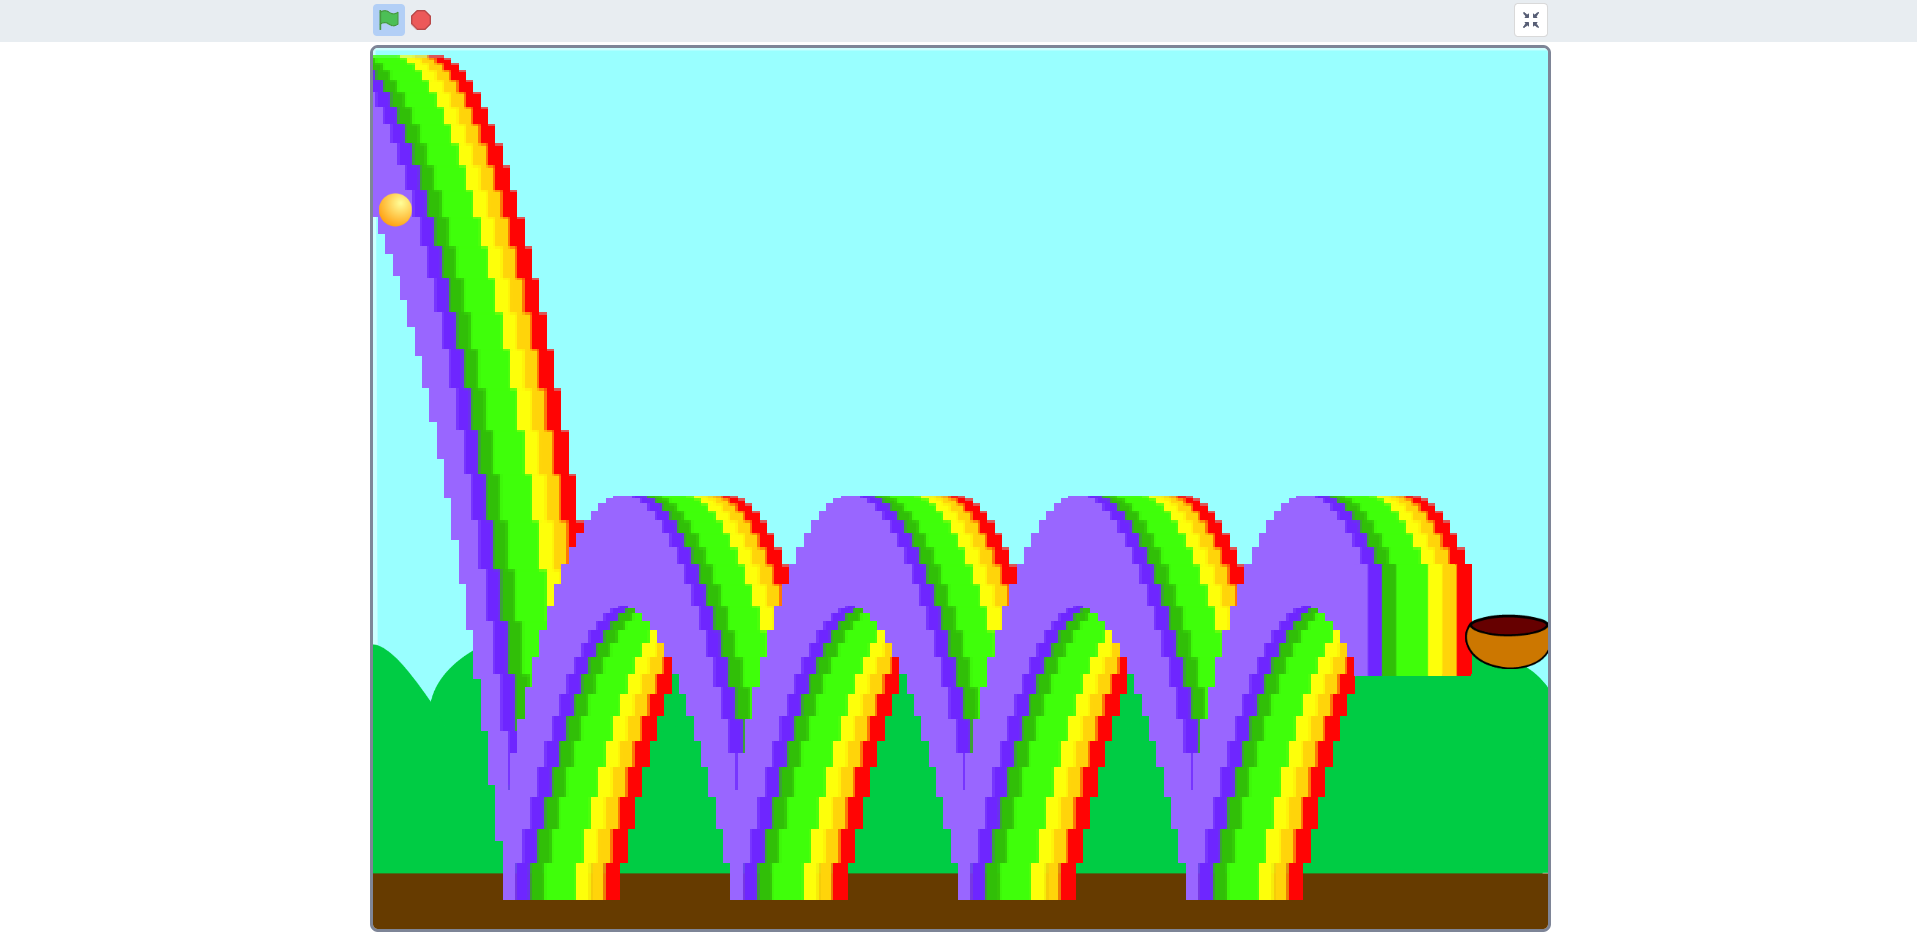
\includegraphics[width=1.0\linewidth,height=0.5\linewidth]{fig070001.png}
  \caption{Скачаща дъга}
\label{fig070001}
\end{figure}

\section{Добавяне на фон и герои}
Първата стъпка от играта е да се добавят подходящ фон и герои. Характерно за фонът е, че трябва да има кафява лента в долната част, която ще служи, като ориентир. Ако фонът, който се избере няма, то тогава може да се добави допълнително, като се използват инструментите за рисуване.

Основният герой не е необходим в тази игра, за това трябва да бъде изтрит. Героите купа и топче са от готовите герои в Scratch. Героят дъга трябва да се нарисува (Фиг. \ref{fig070002}).

\begin{figure}[H]
  \centering
  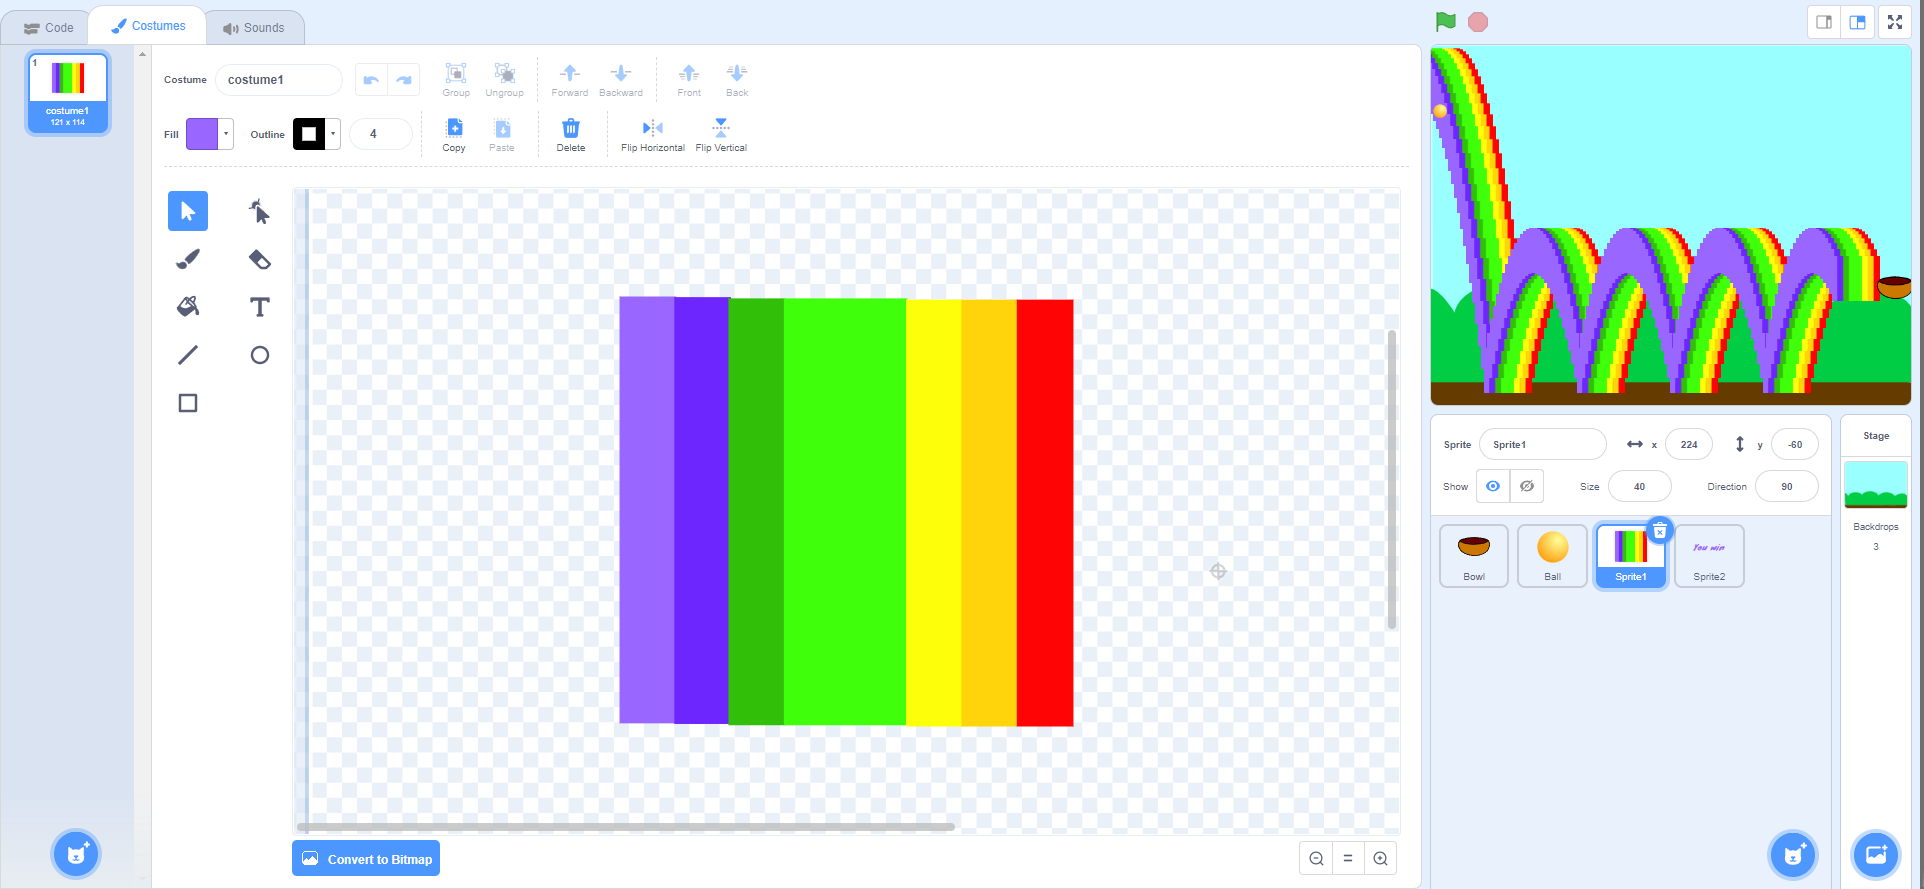
\includegraphics[width=1.0\linewidth,height=0.5\linewidth]{fig070002.png}
  \caption{Добавяне на героя дъга}
\label{fig070002}
\end{figure}

Още един герой трябва да бъде нарисуван. Това е надписа, който ще се появи, когато топчето докосне купата, т.е. играчът успешно премине през цялата дъга.

\begin{figure}[H]
  \centering
  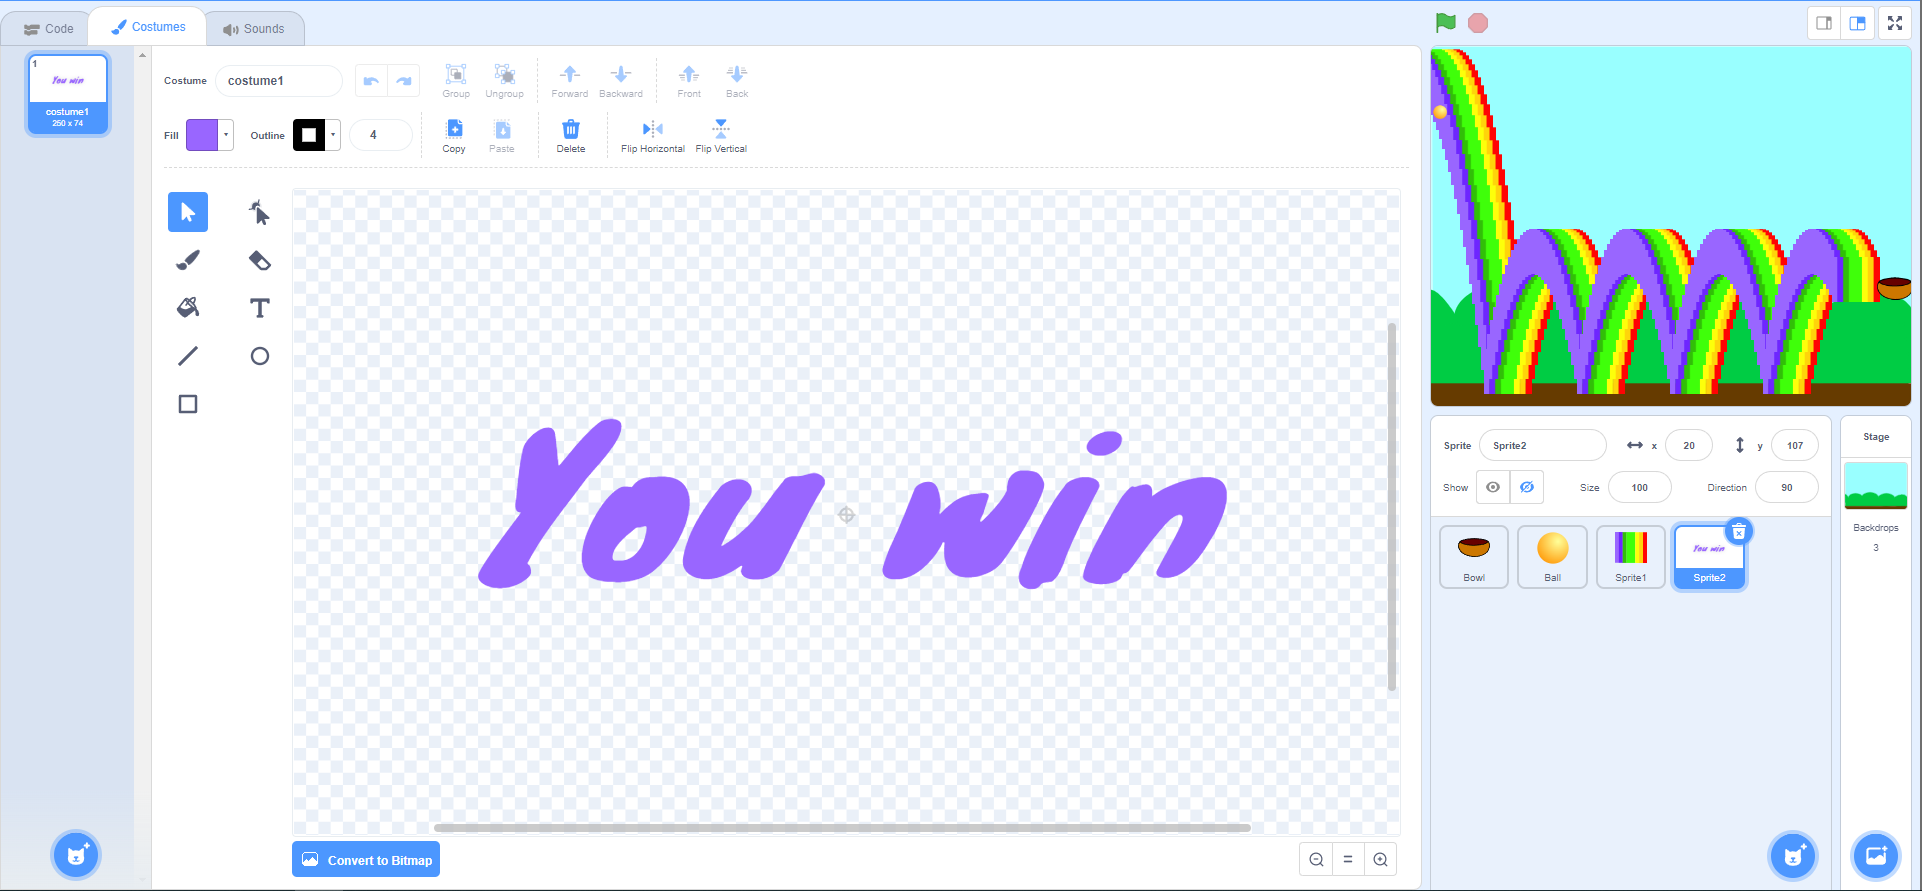
\includegraphics[width=1.0\linewidth,height=0.5\linewidth]{fig070003.png}
  \caption{Добавяне на героя за край на играта}
\label{fig070003}
\end{figure}

\section{Програмиране на купата}
Първите инструкции, които ще се конструират са тези за купата. Нейната цел е да отиде от лявата страна на екрана до дясната подскачайки. Алгоритъмът, който трябва да се конструира за ефекта на подскачане изисква създаване на променлива. В тази променлива ще се съдържа стойността, с която ще се променя координатата y. Докато купата не докосне кафявата граница променливата ще намалява с 1. Когато докосне границата, тогава ще приема стойност 15.

Когато играта започне позицията на купата трябва да бъде в лявата част на екрана. Това означава, че стойността на координатата x трябва да бъде -199, а тази на координатата Y 148. Първоначалната стойност на променливата "velocity" трябва да бъде равна на 0. Размерът на героя трябва да бъде променен да бъде по- малък.

\begin{figure}[H]
  \centering
  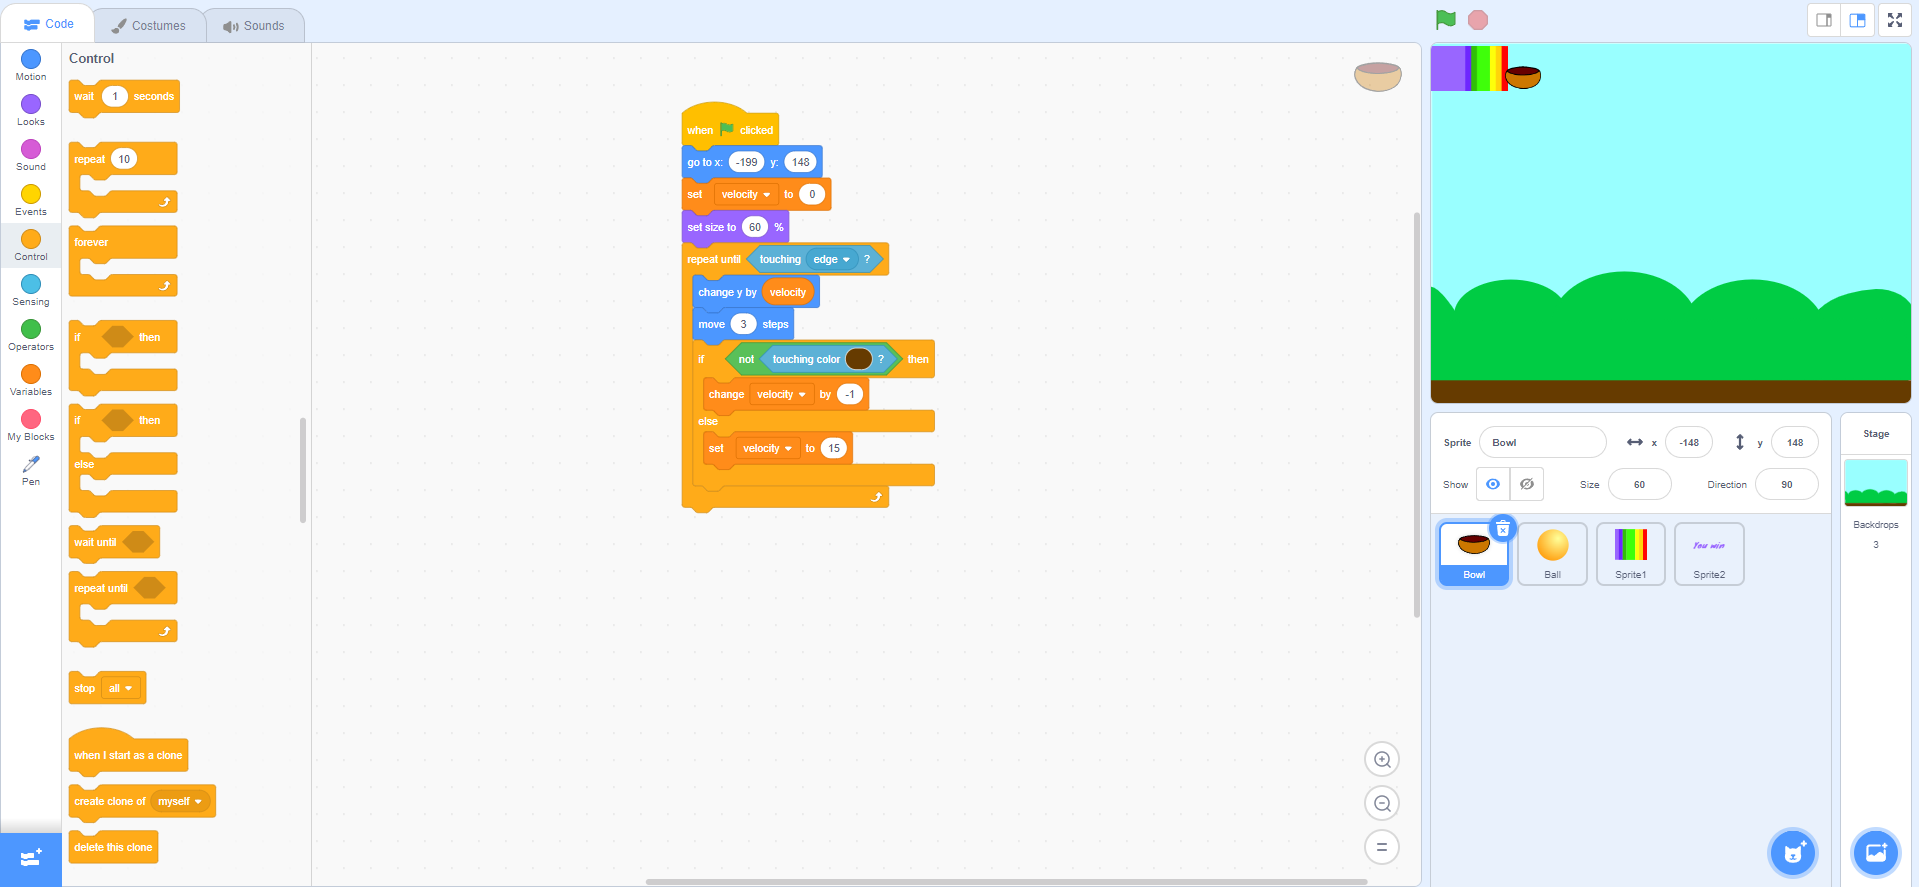
\includegraphics[width=1.0\linewidth,height=0.5\linewidth]{fig070004.png}
  \caption{Позиция на героя купа}
\label{fig070004}
\end{figure}

Следва да се програмира движението на купата. Това движение трябва да се повтаря, което означава, че трябва да се добави цикъл с цел, която е "докато героят не докосне ръб". Това означава, че героят ще се движи, докато не докосне дясната част на екрана. Освен да се движи героят с инструкцията за движение с 3 стъпки, той трябва да променя и y координатата си със стойността на променливата "velocity".

Следва да се добави конструкцията if/else, за да се провери дали героят докосва кафявата граница. Ако не я докосва, то трябва да се намали променливата, за да се премести героя надолу. Ако докосне границата - променливата трябва да има стойност 15. За да се направи проверката, че не се докосва кафявия цвят трябва да се добави инструкция за отрицание, която се намира в зелената група. Проверката за цвят е в светло синята група. За да се намери точния цвят се използва инструмента пипетка, като се постави на кафявия цвят. Чрез инструкции алгоритъмът за движение изглежда така:

\begin{figure}[H]
  \centering
  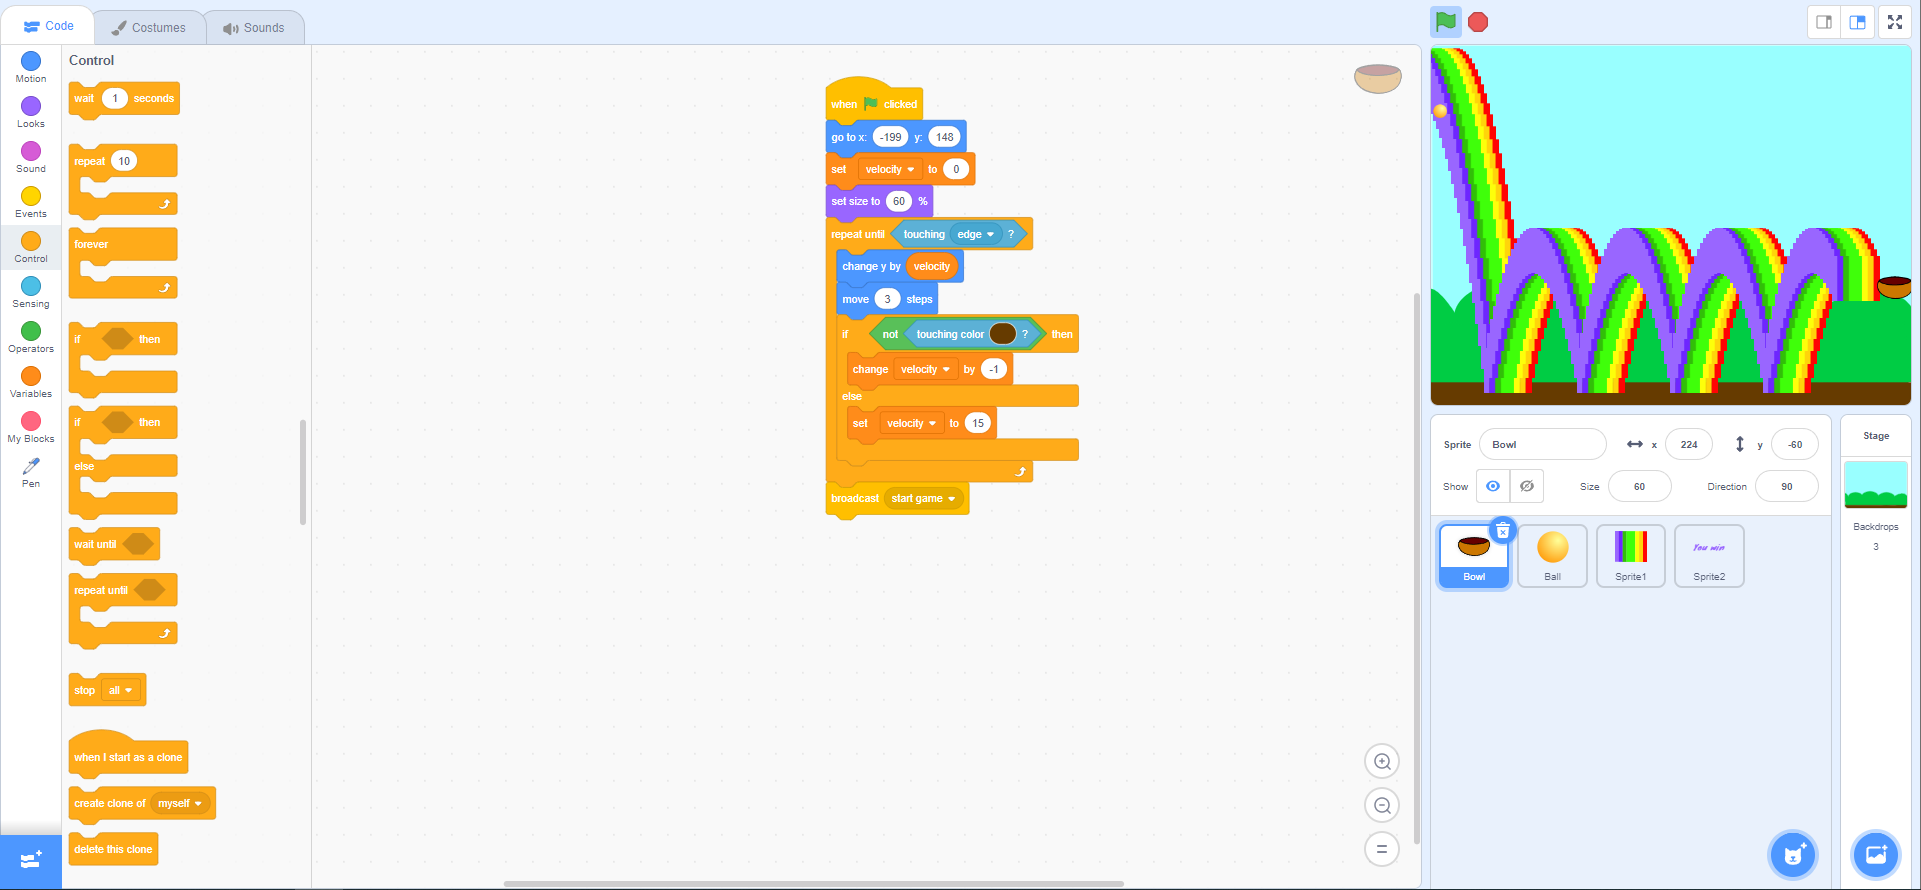
\includegraphics[width=1.0\linewidth,height=0.5\linewidth]{fig070005.png}
  \caption{Движение на героя купа}
\label{fig070005}
\end{figure}

След като героят достигне целта си, той трябва да изпрати съобщение "start game". Чак тогава играта може да започне. Инструкцията за изпращане на съобщения се намира в жълтата група с инструкции.

\begin{figure}[H]
  \centering
  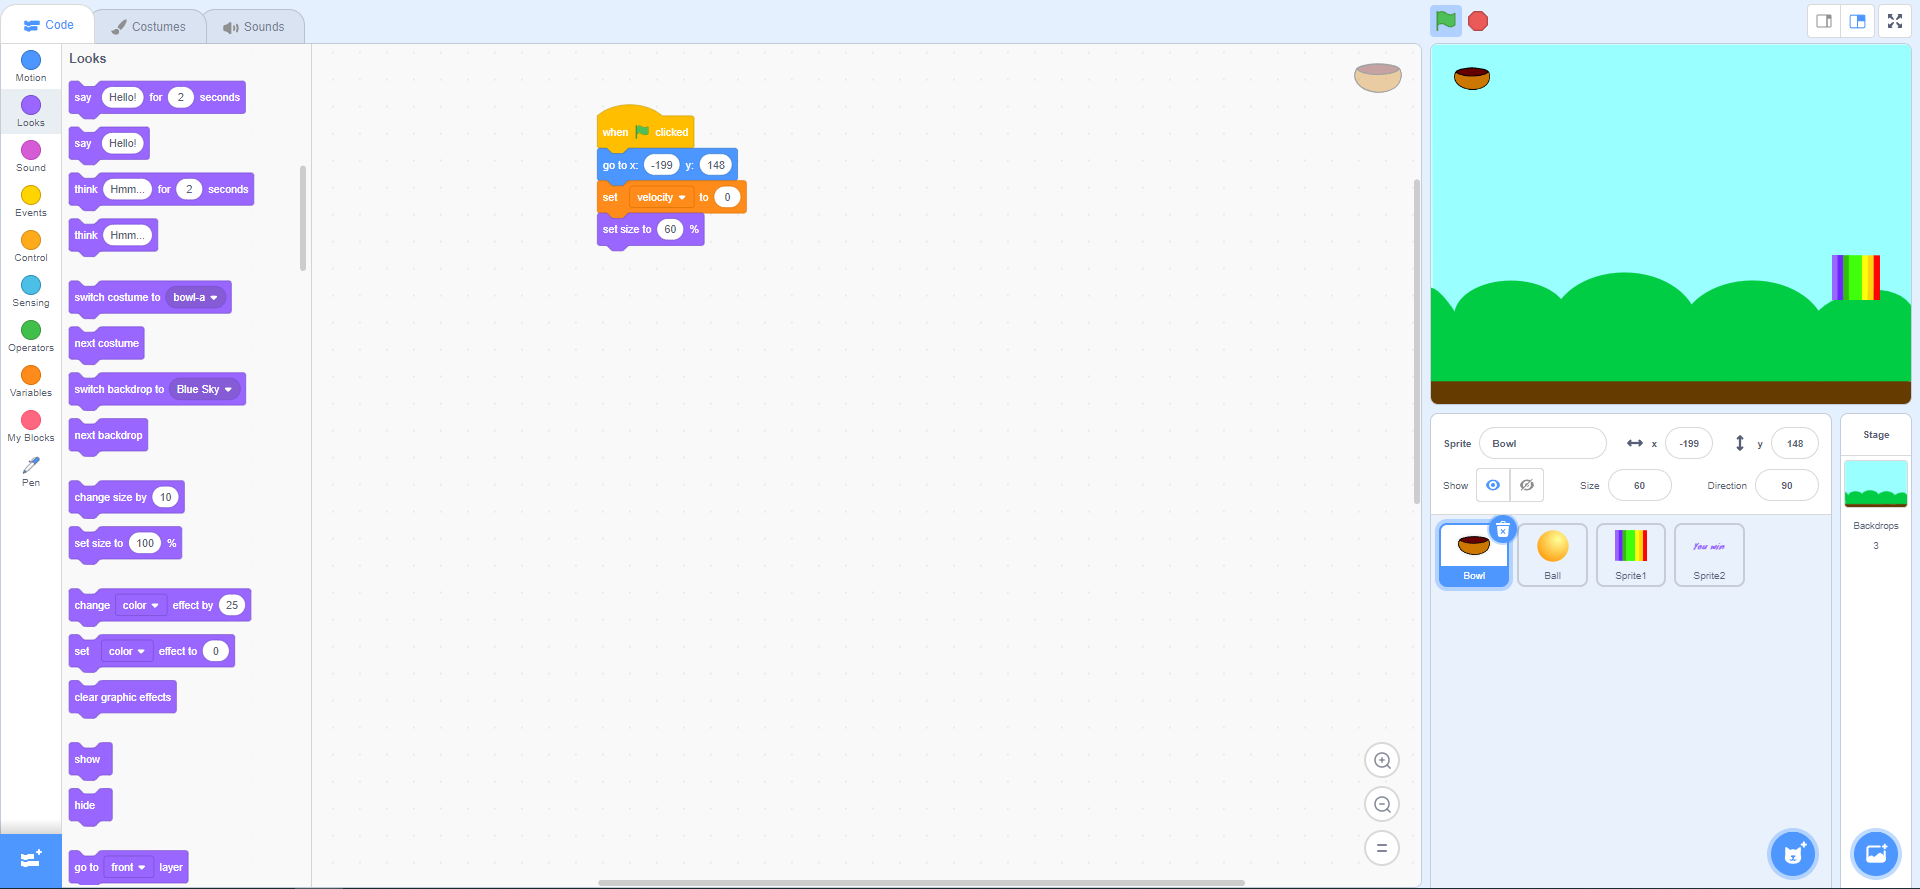
\includegraphics[width=1.0\linewidth,height=0.5\linewidth]{fig070006.png}
  \caption{Кодът героя купа}
\label{fig070006}
\end{figure}

Когато се стартира играта се забелязва, че героят преминава от едната част на екрана до другата, подскачайки.

\section{Програмиране на дъгата}
За да се програмира този герой да оставя следи трябва да се добави нова група с инструкции - Pen.

\begin{figure}[H]
  \centering
  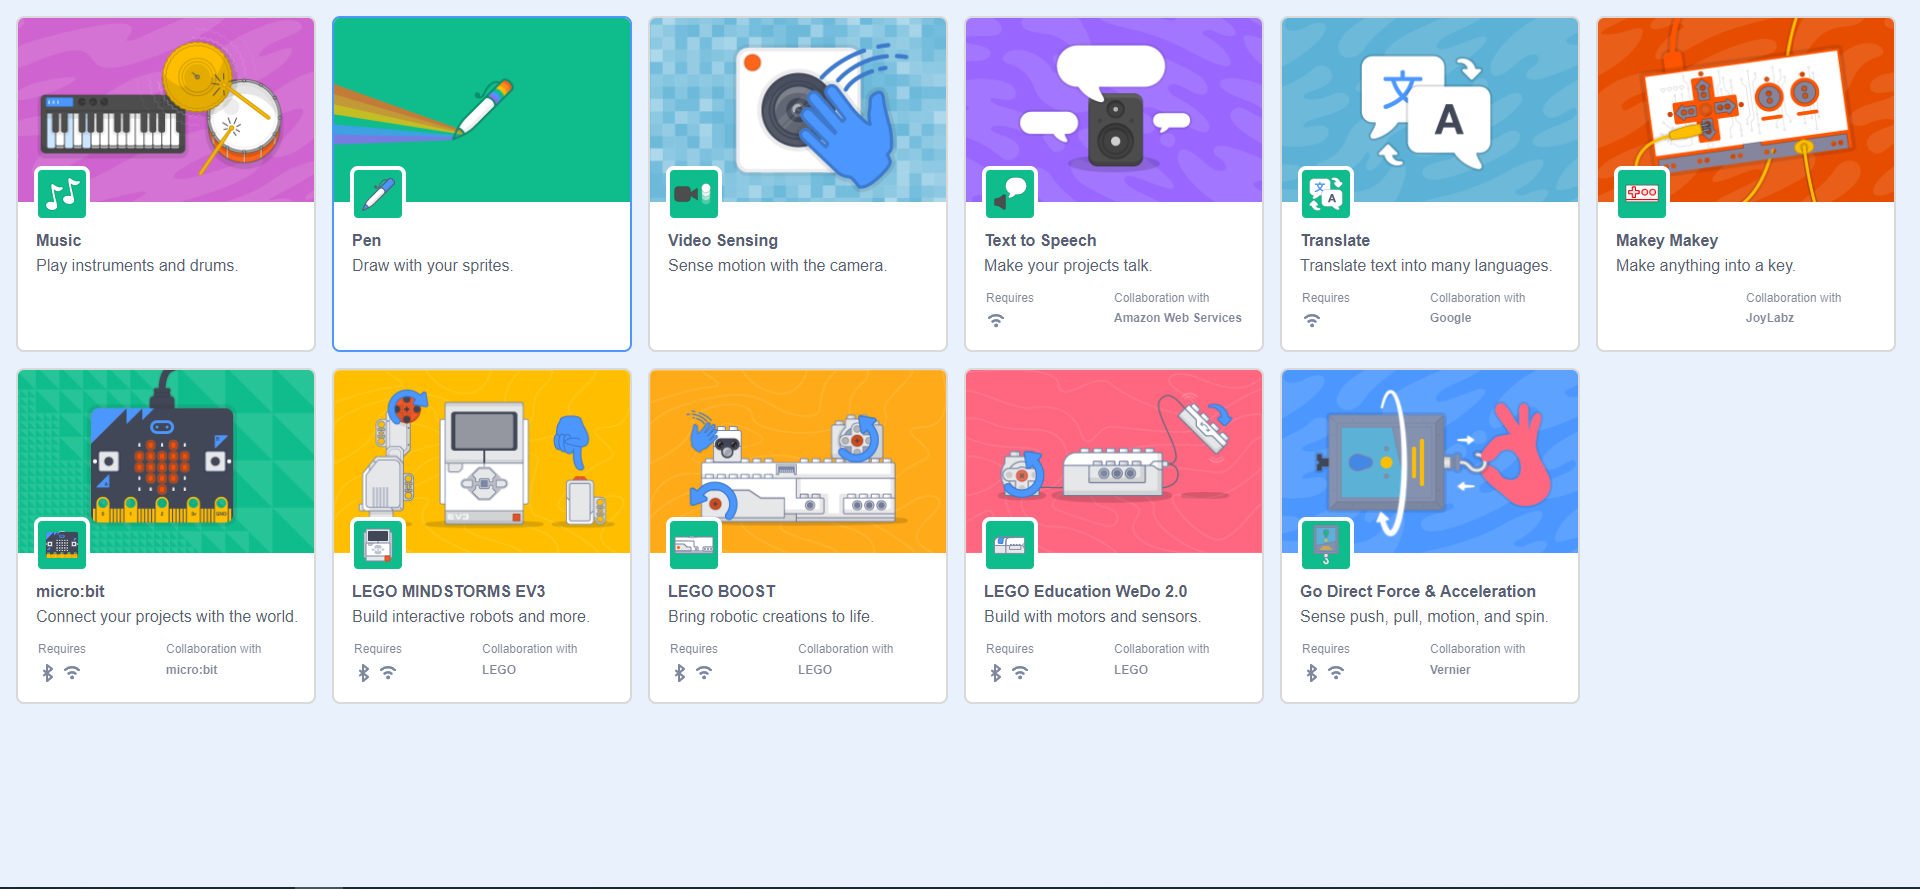
\includegraphics[width=1.0\linewidth,height=0.5\linewidth]{fig070007.png}
  \caption{Нова група инструкции Pen}
\label{fig070007}
\end{figure}

Спрямо това как е нарисуван героят, трябва да се намали. Това може да стане и без инструкции, а като се промени свойството Size.

\begin{figure}[H]
  \centering
  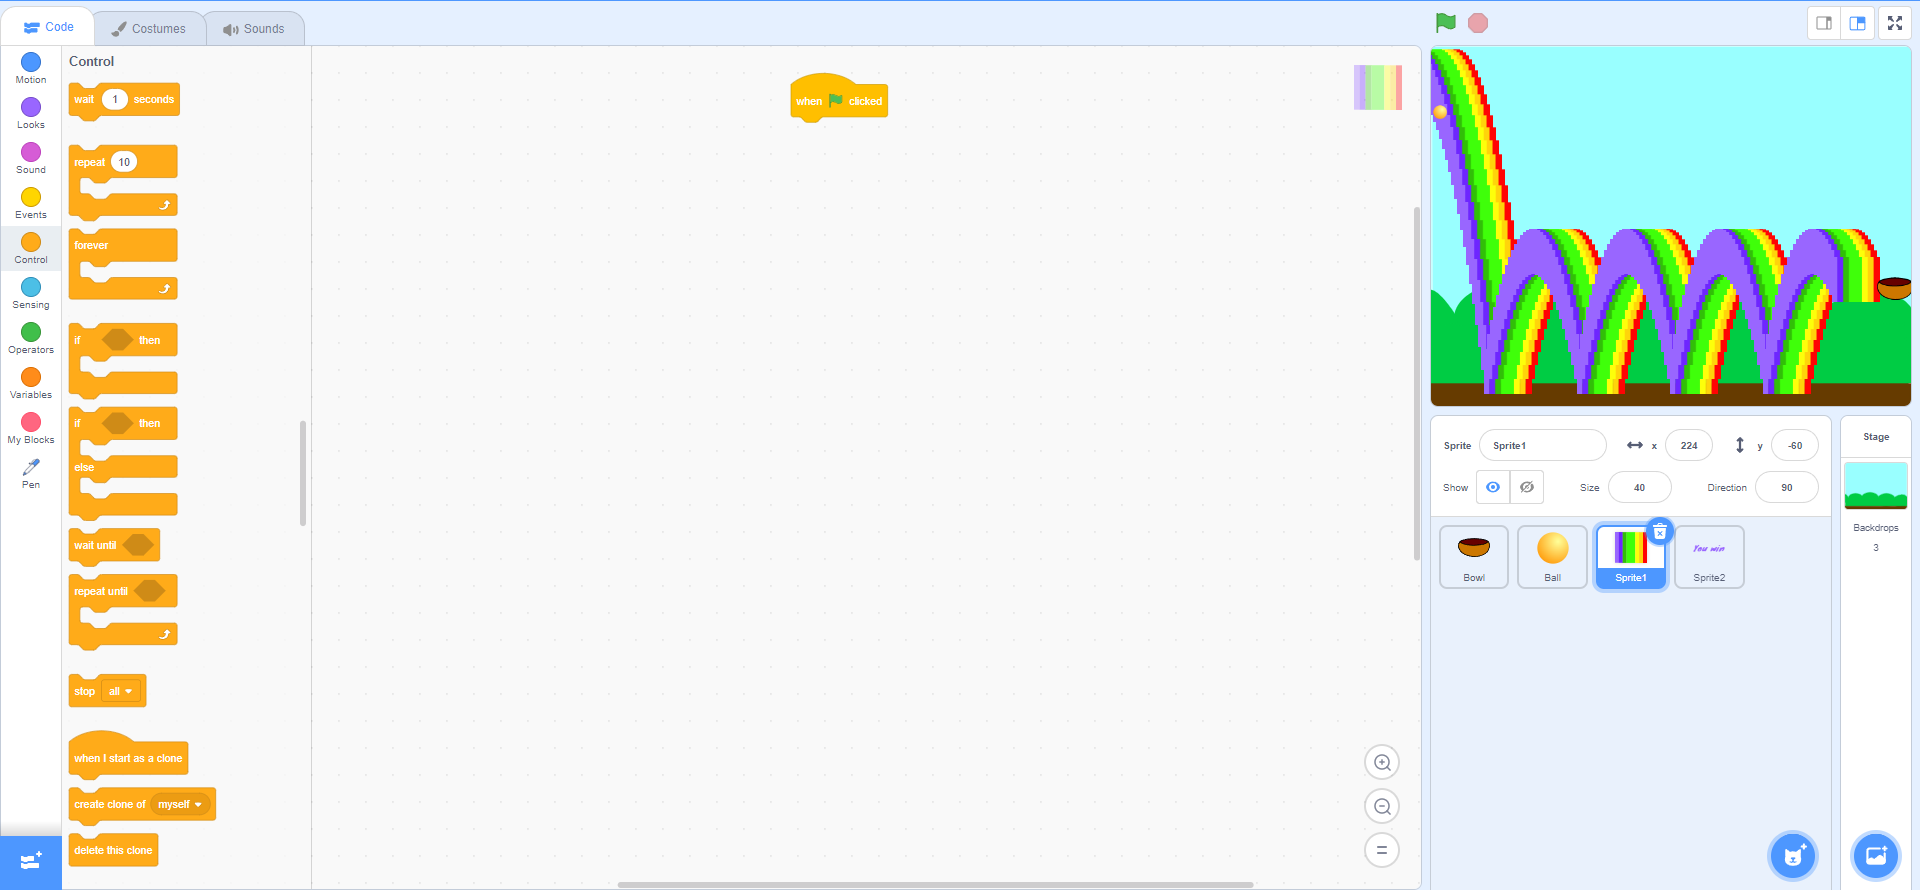
\includegraphics[width=1.0\linewidth,height=0.5\linewidth]{fig070008.png}
  \caption{Промяна на свойството Size}
\label{fig070008}
\end{figure}

Инструкциите на този герой са единствено да следва героя купа и да оставя следи. В началото на играта всичко нарисувано трябва да бъде изтрито. Това става с помощта на инструкцията "erase all", която се намира в новата добавена група с инструкции. Дъгата освен да следва движението на героя купа, трябва да следва и неговата посока. Това става с помощта на инструкцията от синята група "point in direction". За да се укаже коя точно посока да следва, трябва да се използва инструкция от светлосинята група, която е "backdrop of Stage". Първо се променя втората стойност от "Stage" на името на героя. След това се променя и вида, който трябва да бъде "direction".

\begin{figure}[H]
  \centering
  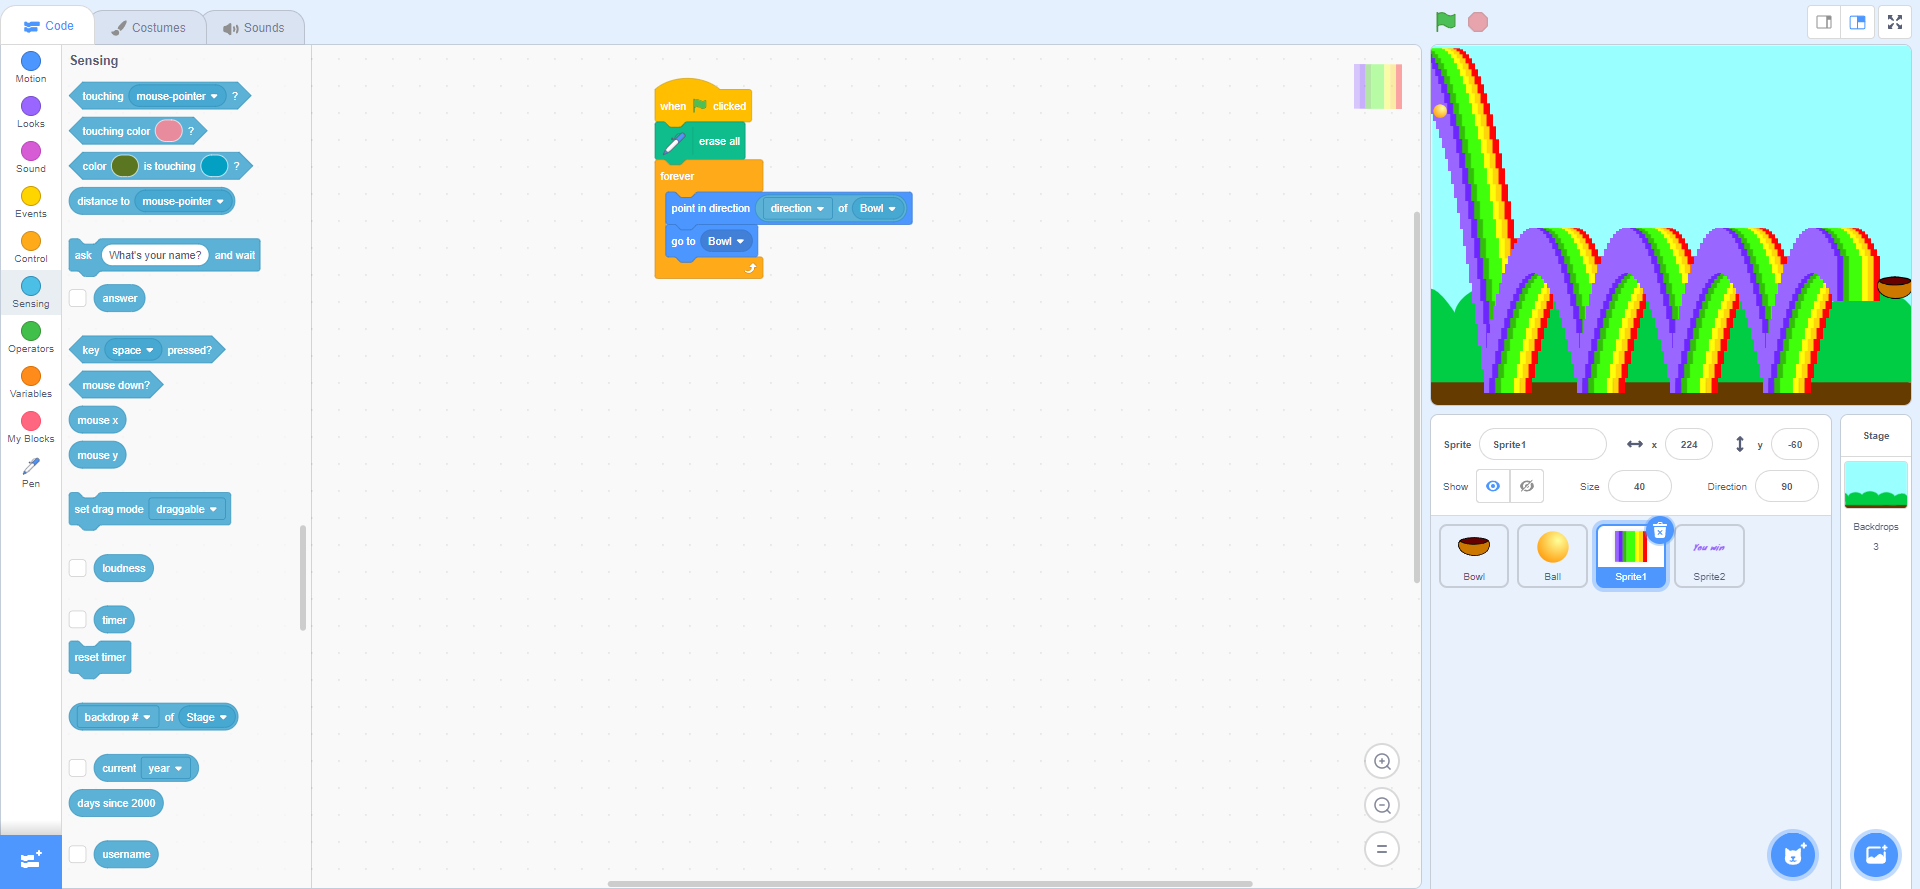
\includegraphics[width=1.0\linewidth,height=0.5\linewidth]{fig070009.png}
  \caption{Движение на героя дъга}
\label{fig070009}
\end{figure}

Ако се стартира програмата се забелязва, че героят дъга само следва героя купа. За да оставя следа, трябва да се използва инструкцията "stamp", която се намира в новата група.

\begin{figure}[H]
  \centering
  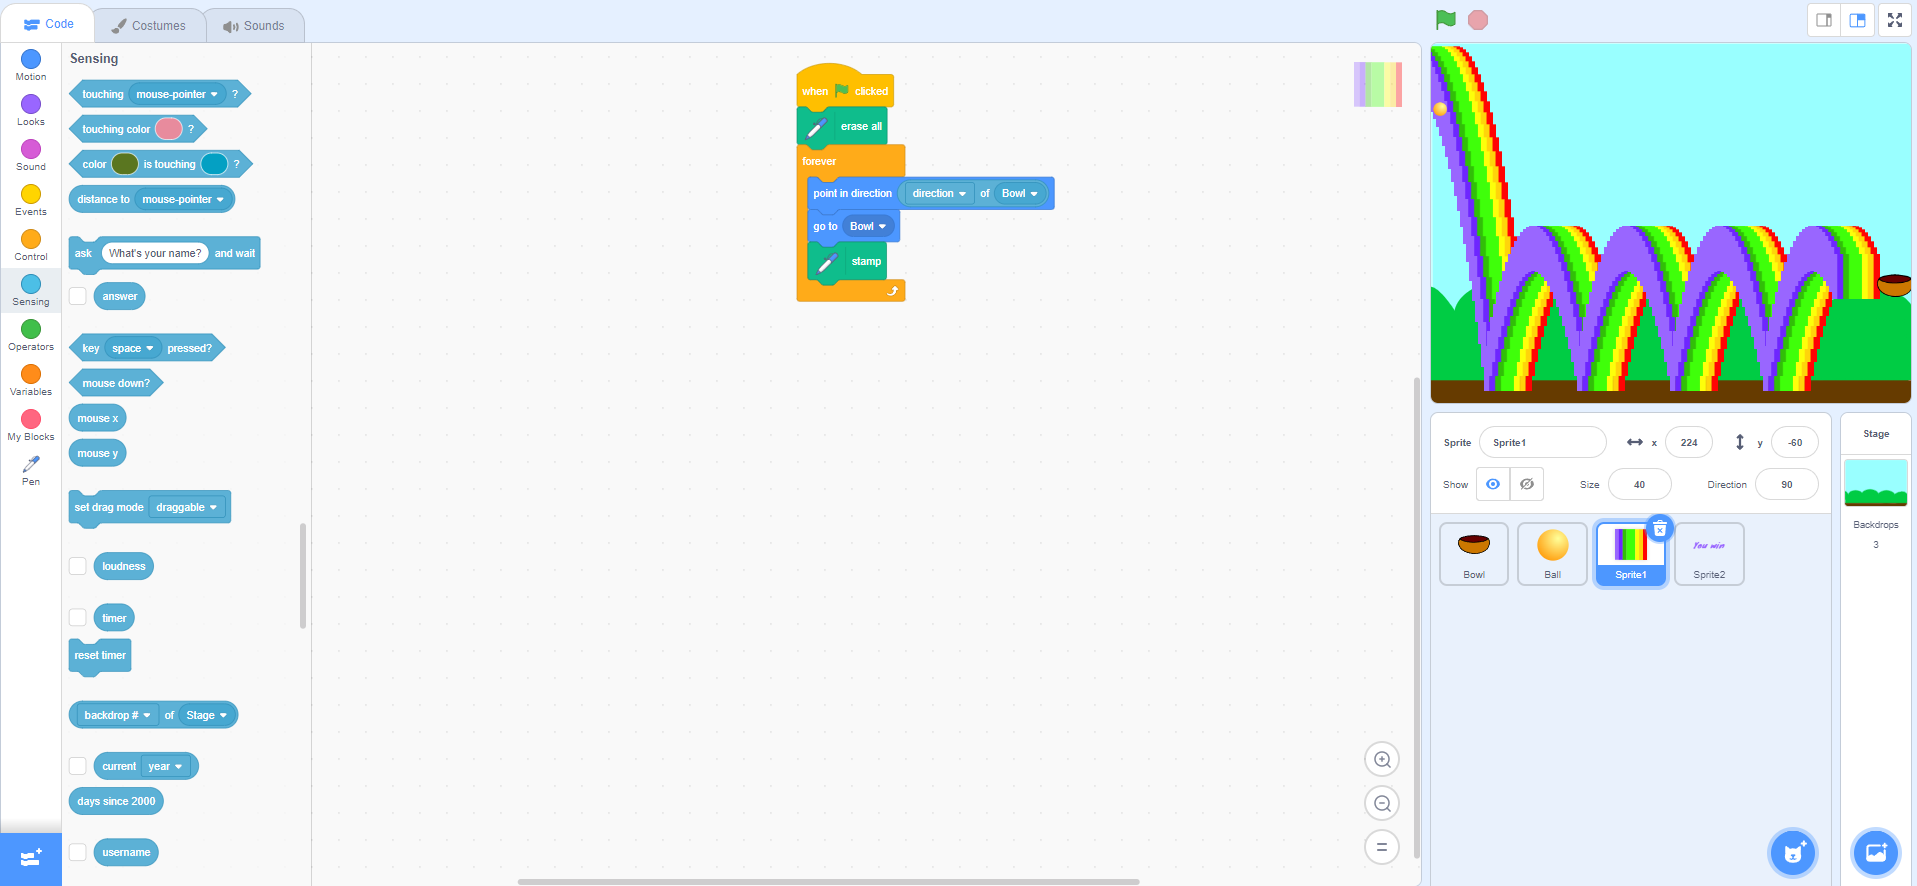
\includegraphics[width=1.0\linewidth,height=0.5\linewidth]{fig070010.png}
  \caption{Целия код на героя дъга}
\label{fig070010}
\end{figure}

\section{Програмиране на топчето}
Размерите на топчето трябва да бъдат такива, че то да може да преминава през цялата дъга докосвайки лилавия (или най- външния) цвят. Те могат да се променят, като се промени стойността на свойството Size.

\begin{figure}[H]
  \centering
  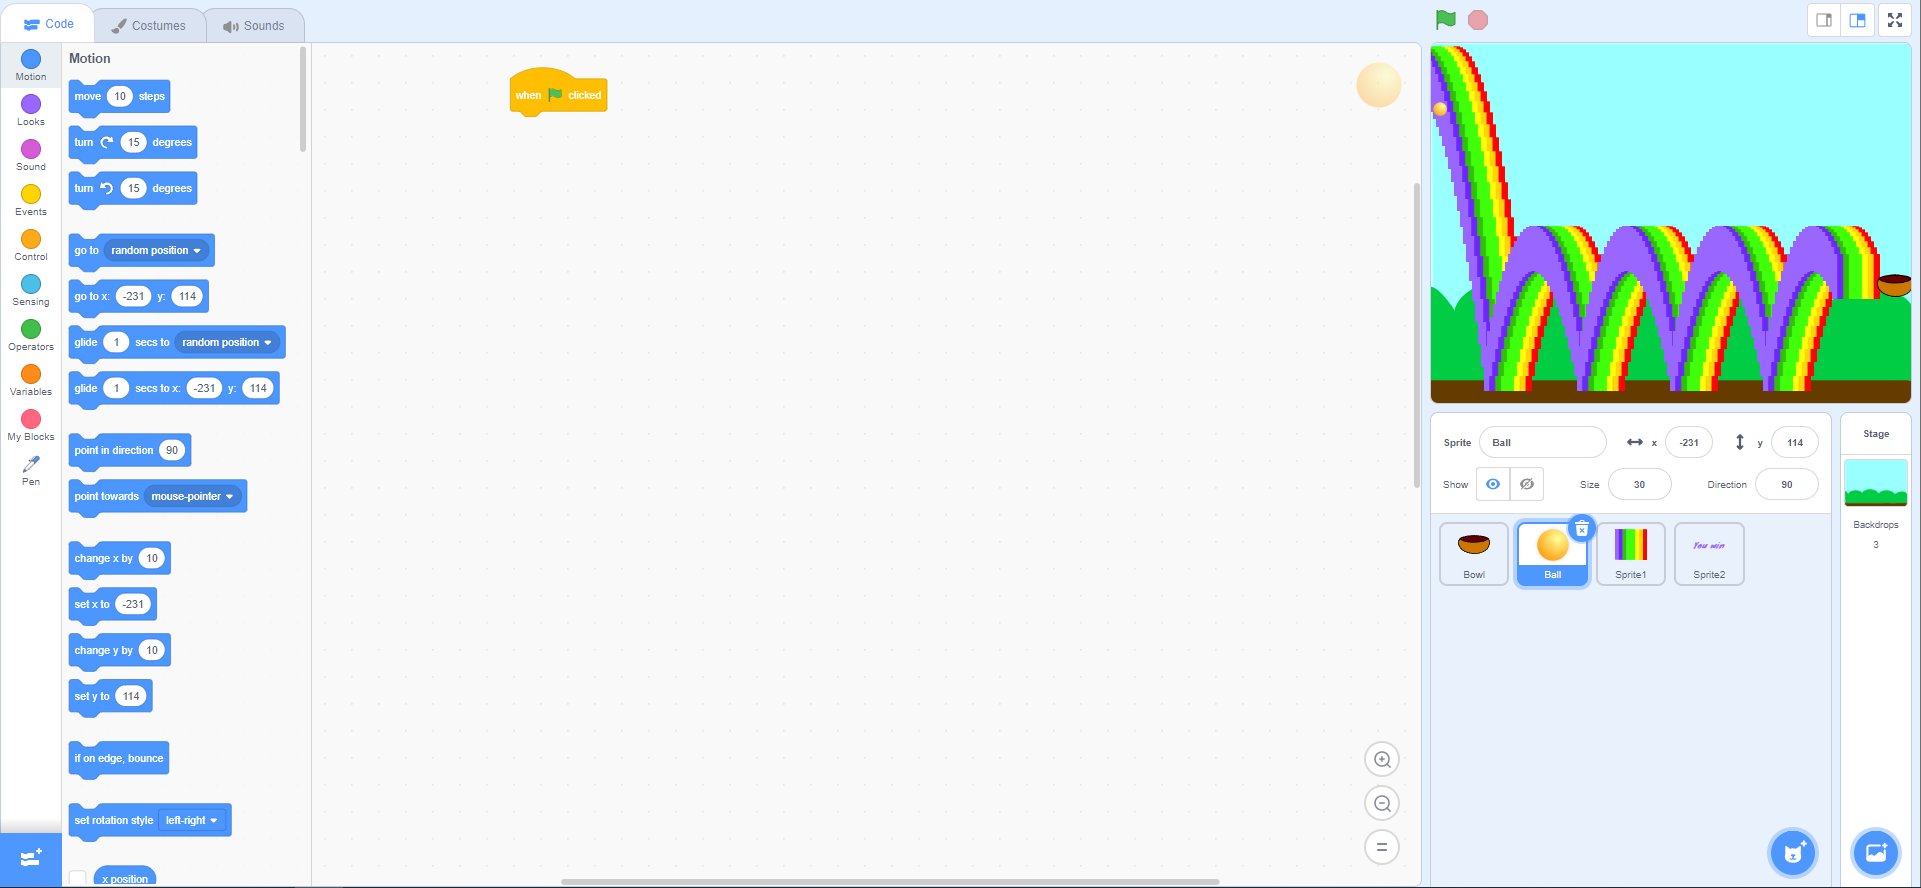
\includegraphics[width=1.0\linewidth,height=0.5\linewidth]{fig070011.png}
  \caption{Размер на героя топче}
\label{fig070011}
\end{figure}

Топчето трябва да се появи, когато купата стигне до края на екрана. Чрез инструкции това означава, когато героят получи съобщението "start game", тогава се появява. Когато се натисне зеления флаг, то трябва да се скрие. Когато се покаже, може да се направи лека анимация, за да се премести на позиция с координати за x=-231, а за y=114.

\begin{figure}[H]
  \centering
  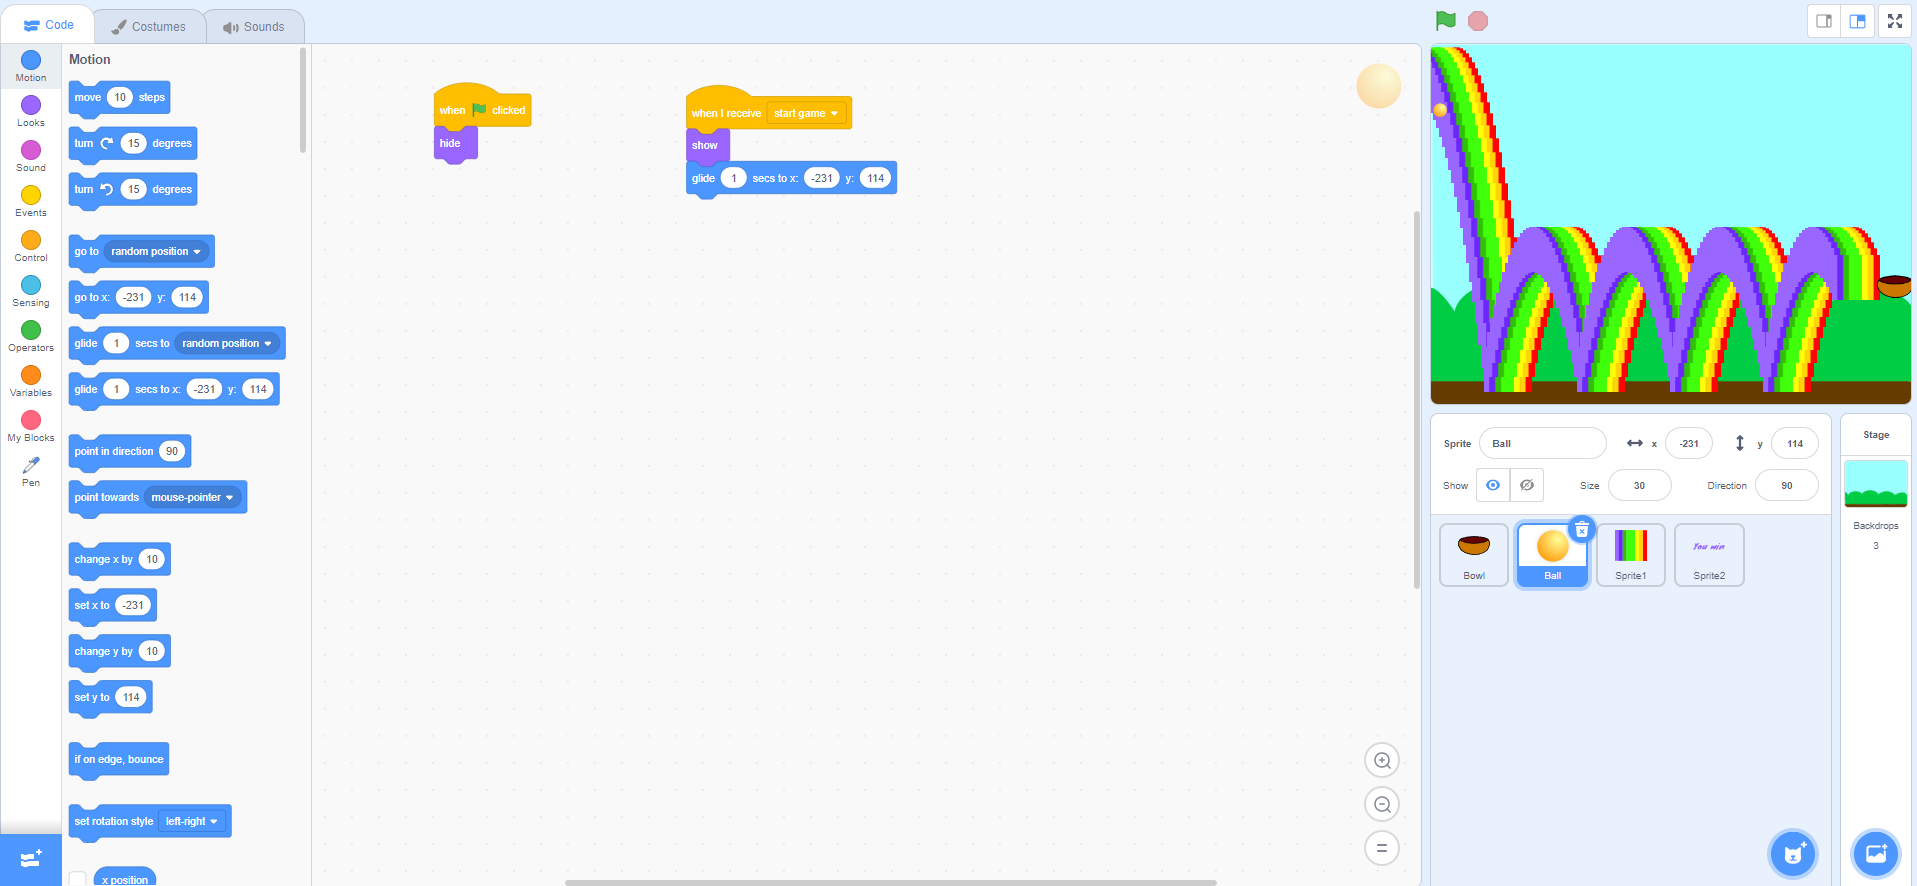
\includegraphics[width=1.0\linewidth,height=0.5\linewidth]{fig070012.png}
  \caption{Начална позиция на героя топче}
\label{fig070012}
\end{figure}

Героят трябва да започне да се движи, когато бъде натиснат. Той се движи докато докосва най- крайния цвят - в случая лилавия. Отново трябва да се ползва цикъл с цел. Целта трябва да бъде "докато спреш да докосваш лилавия цвят". Инструкциите извън цикълът ще се изпълнят, когато условието бъде лъжа. В този случай означава, когато героят не докосва дъгата, тогава се премести в начална позиция.

Инструкцията за движение трябва да бъде - следвай мишката. Тази инструкция се намира в синята група с инструкции и е go to mouse-pointer. Ако се наложи героят да се движи по- бавно, това става, като се добави инструкцията за изчакване от оранжевата група.

\begin{figure}[H]
  \centering
  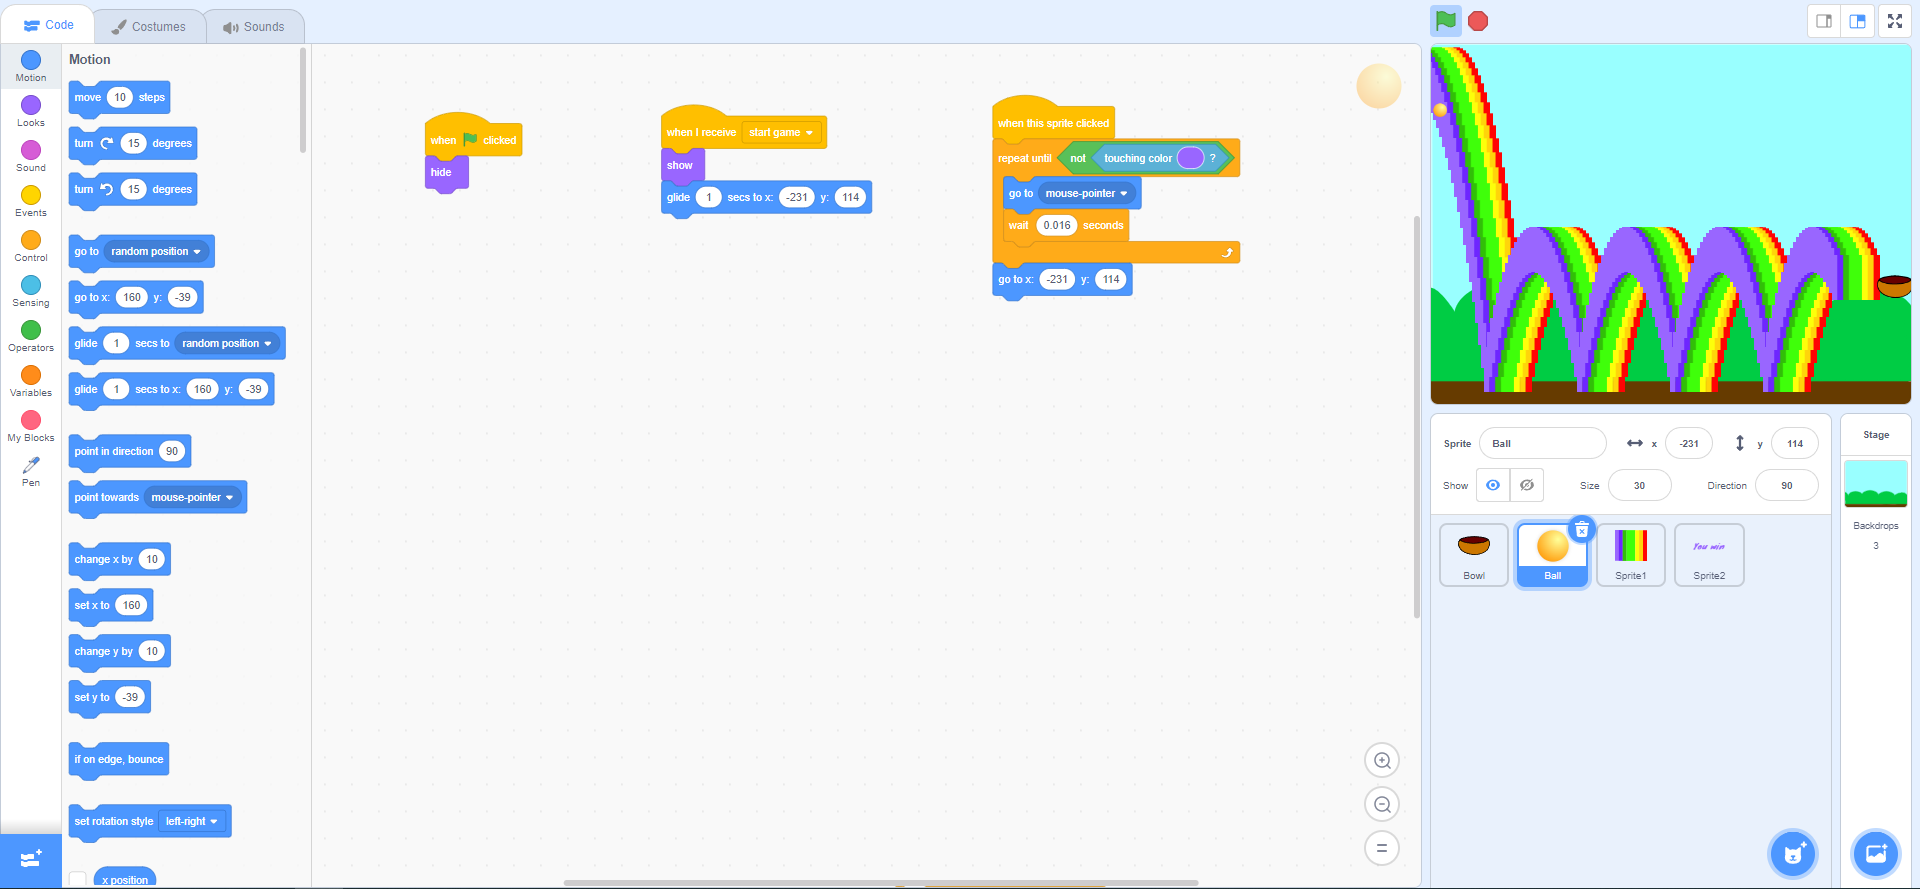
\includegraphics[width=1.0\linewidth,height=0.5\linewidth]{fig070013.png}
  \caption{Движение на героя топче}
\label{fig070013}
\end{figure}

Последното нещо, което трябва да се направи е проверка за това дали героят е достигнал края на дъгата. Ако е, тогава ще изпрати съобщение на героя, който е надпис да се появи и играта да приключи. В края на дъгата се намира героя дъга. Тогава проверката за това дали да приключи играта е много лесна - докоснало ли е топчето дъгата. Ако е - изпраща съобщение и приключва играта. Ако не е - играта продължава.

\begin{figure}[H]
  \centering
  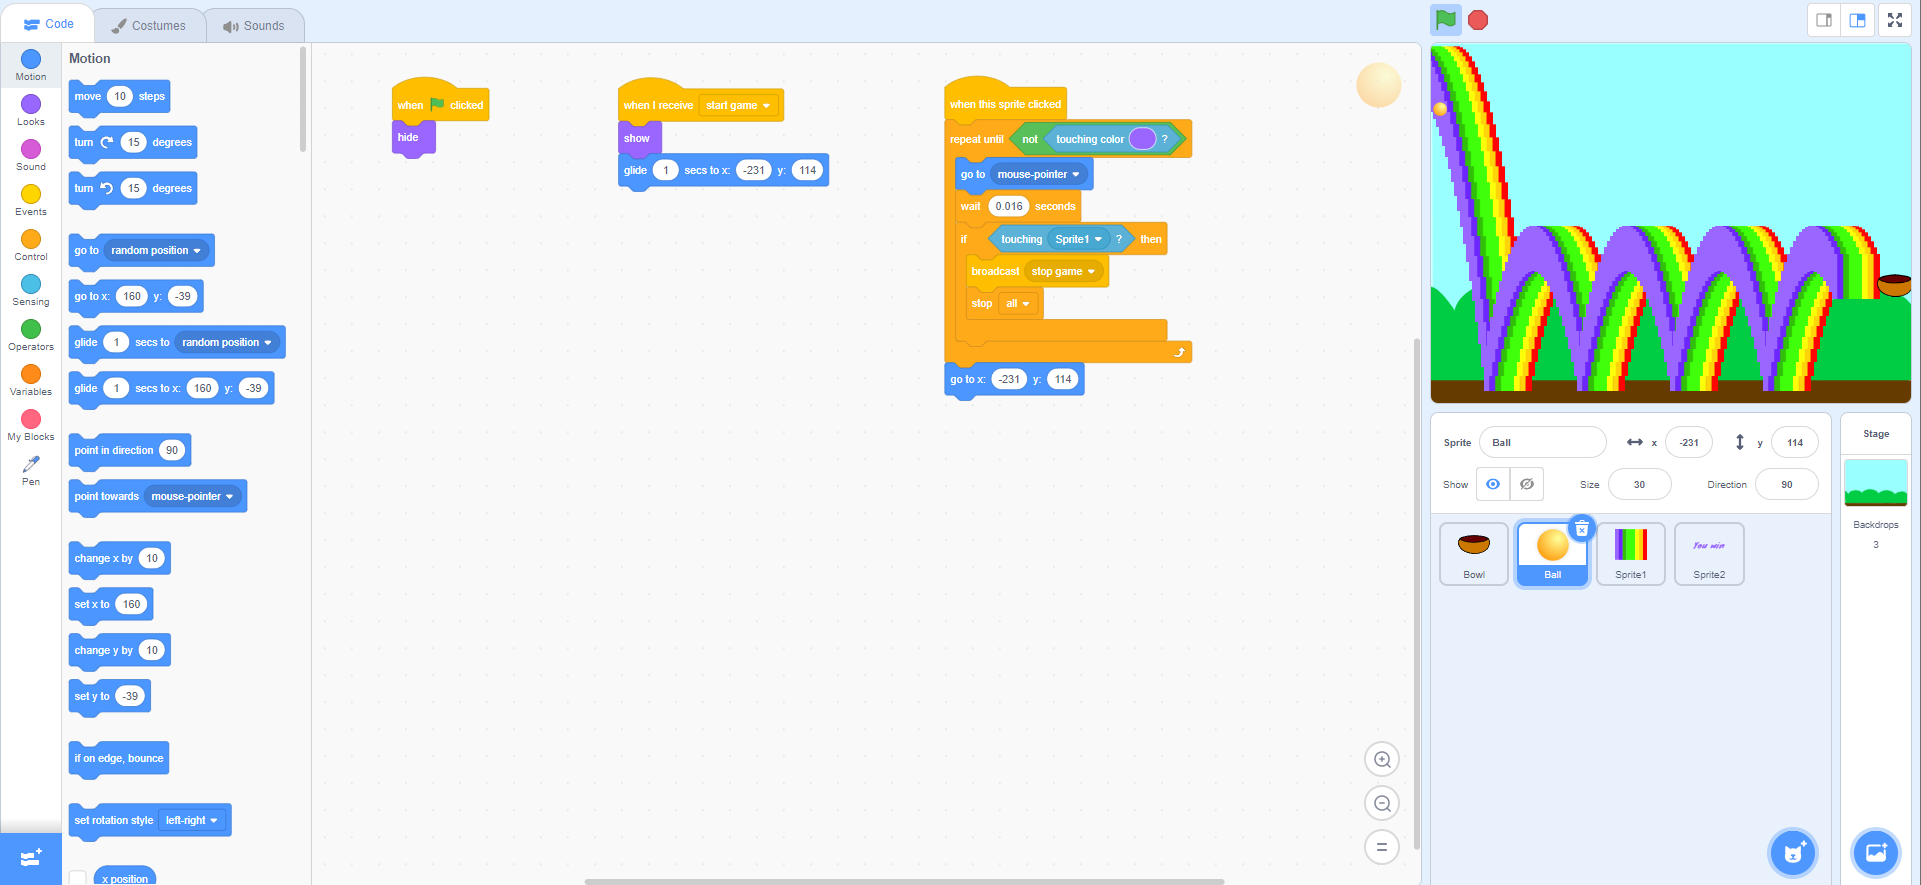
\includegraphics[width=1.0\linewidth,height=0.5\linewidth]{fig070014.png}
  \caption{Кодът на героя топче}
\label{fig070014}
\end{figure}

\section{Край на играта}
Героят, който е надписа за край на играта трябва да бъде скрит в началото. Той се появява, когато топчето изпрати съобщение за край на играта.

\begin{figure}[H]
  \centering
  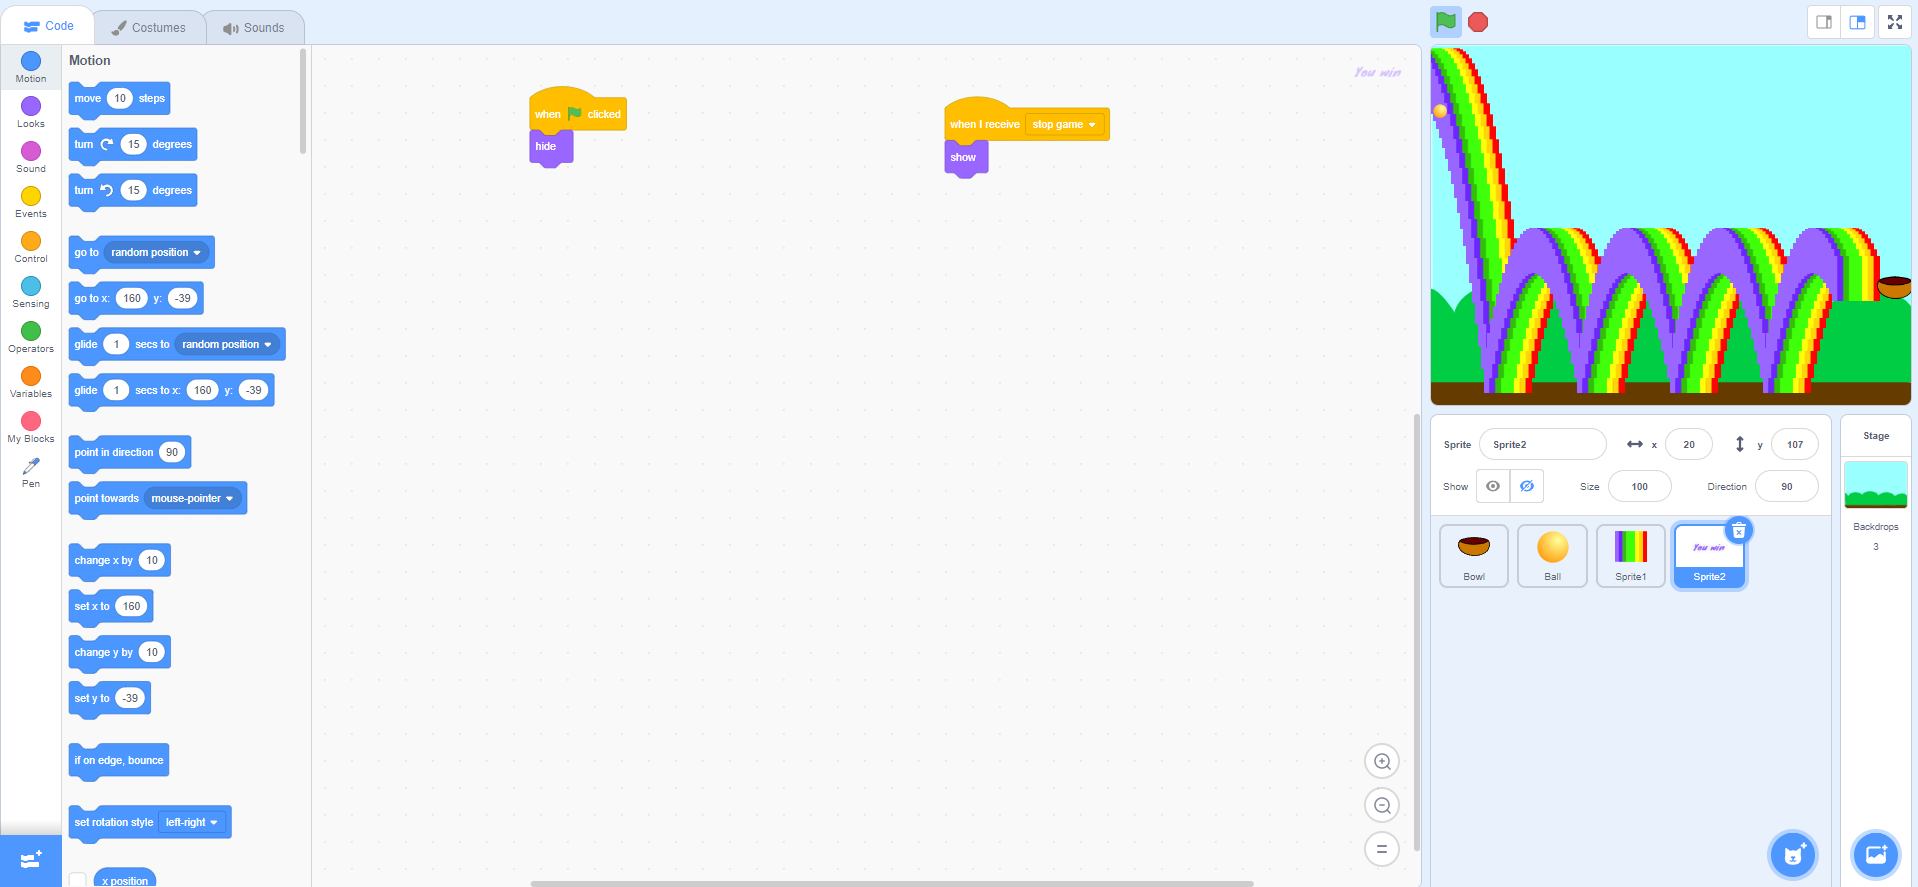
\includegraphics[width=1.0\linewidth,height=0.5\linewidth]{fig070015.png}
  \caption{Кодът на героя надпис}
\label{fig070015}
\end{figure}